\documentclass[10pt, onecolumn]{article}
\usepackage{amsmath}
\usepackage{enumerate}
\usepackage{enumitem}
\usepackage{listings}
\usepackage[utf8]{inputenc}
\usepackage{amssymb}
\usepackage{tabularx}
\usepackage{tikz}
\usetikzlibrary{arrows,positioning,shapes.geometric}
\usepackage{booktabs}
\usepackage{multirow}
\usepackage{siunitx}
\usepackage{graphicx}
\graphicspath{{./images/}}
\lstset{
    frame=single,
    breaklines=true
}
\usepackage{hyperref}
%\usepackage{atbegshi}
%\AtBeginDocument{\AtBeginShipoutNext{\AtBeginShipoutDiscard}}
%\newcommand{\solution}{\noindent \textbf{Solution:}}
%\documentclass[twoside]{article}
\usepackage[a4paper,outer=1.5cm,inner=1.5cm,top=1.75cm,bottom=1.5cm]{geometry}
\def\mytitle{\textbf{CHANNEL DECODING}}
\def\myauthor{TUNGALA SIVA PARVATHI}
\def\contact{tvssn143@gmail.com}
%\def\myauthor{}
\def\contact{tvssn143@gmail.com }
\def\mymodule{Future Wireless Communication (FWC)}

%\thiswatermark{\centering \put(-15,-100.0){\includegraphics[scale=0.4]{iith.png}} }
\title{\mytitle}
\author{\myauthor\hspace{1em}\\\contact\\FWC22089 -\hspace{0.5em}IITH\hspace{0.5em}\mymodule\hspace{6em}}

\begin{document}
\maketitle
\section{Definition}
Channel decoding in NAVIC, the Indian Regional Navigation Satellite System, involves the process of error correction and retrieval of the original data transmitted over the satellite link. The channel decoding scheme used in NAVIC is based on a convolutional coding technique known as Rate 1/2 Convolutional Code with Viterbi decoding.
\subsection{Process}
Here is a high-level description of the channel decoding process in NAVIC:


\tikzset{every picture/.style={line width=0.75pt}} %set default line width to 0.75pt        

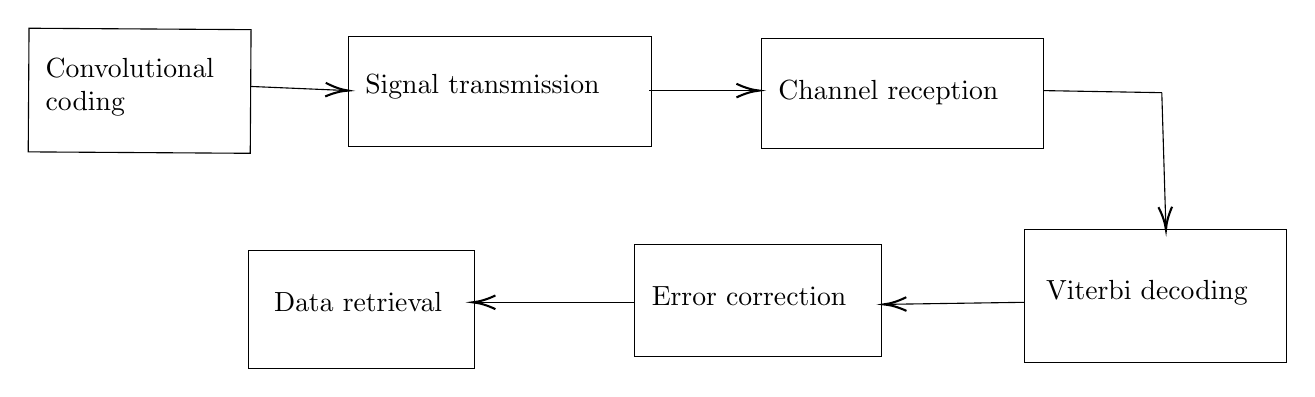
\begin{tikzpicture}[x=0.75pt,y=0.75pt,yscale=-1,xscale=1]
%uncomment if require: \path (0,300); %set diagram left start at 0, and has height of 300

%Shape: Rectangle [id:dp47147121431531436] 
\draw   (25.24,20.95) -- (132.21,21.64) -- (131.82,81.21) -- (24.85,80.52) -- cycle ;
%Shape: Rectangle [id:dp6699181989834492] 
\draw   (179,25) -- (325,25) -- (325,78) -- (179,78) -- cycle ;
%Shape: Rectangle [id:dp13625380852022662] 
\draw   (378,26) -- (514,26) -- (514,79) -- (378,79) -- cycle ;
%Shape: Rectangle [id:dp7604816059628322] 
\draw   (505,118) -- (631,118) -- (631,182) -- (505,182) -- cycle ;
%Shape: Rectangle [id:dp09128390751102777] 
\draw   (317,125) -- (436,125) -- (436,179) -- (317,179) -- cycle ;
%Shape: Rectangle [id:dp3624421410733156] 
\draw   (131,128) -- (240,128) -- (240,185) -- (131,185) -- cycle ;
%Straight Lines [id:da7357860930553348] 
\draw    (132,49) -- (177,50.91) ;
\draw [shift={(179,51)}, rotate = 182.44] [color={rgb, 255:red, 0; green, 0; blue, 0 }  ][line width=0.75]    (10.93,-3.29) .. controls (6.95,-1.4) and (3.31,-0.3) .. (0,0) .. controls (3.31,0.3) and (6.95,1.4) .. (10.93,3.29)   ;
%Straight Lines [id:da7059963475403158] 
\draw    (324,51) -- (375,51) ;
\draw [shift={(377,51)}, rotate = 180] [color={rgb, 255:red, 0; green, 0; blue, 0 }  ][line width=0.75]    (10.93,-3.29) .. controls (6.95,-1.4) and (3.31,-0.3) .. (0,0) .. controls (3.31,0.3) and (6.95,1.4) .. (10.93,3.29)   ;
%Straight Lines [id:da1756708396189547] 
\draw    (317,153) -- (241,153) ;
\draw [shift={(239,153)}, rotate = 360] [color={rgb, 255:red, 0; green, 0; blue, 0 }  ][line width=0.75]    (10.93,-3.29) .. controls (6.95,-1.4) and (3.31,-0.3) .. (0,0) .. controls (3.31,0.3) and (6.95,1.4) .. (10.93,3.29)   ;
%Straight Lines [id:da48261577945996814] 
\draw    (505,153) -- (439,153.97) ;
\draw [shift={(437,154)}, rotate = 359.16] [color={rgb, 255:red, 0; green, 0; blue, 0 }  ][line width=0.75]    (10.93,-3.29) .. controls (6.95,-1.4) and (3.31,-0.3) .. (0,0) .. controls (3.31,0.3) and (6.95,1.4) .. (10.93,3.29)   ;
%Straight Lines [id:da2447168448689644] 
\draw    (571,52) -- (572.94,116) ;
\draw [shift={(573,118)}, rotate = 268.26] [color={rgb, 255:red, 0; green, 0; blue, 0 }  ][line width=0.75]    (10.93,-3.29) .. controls (6.95,-1.4) and (3.31,-0.3) .. (0,0) .. controls (3.31,0.3) and (6.95,1.4) .. (10.93,3.29)   ;
%Straight Lines [id:da4570154485730509] 
\draw    (514,51) -- (571,52) ;

% Text Node
\draw (32,34) node [anchor=north west][inner sep=0.75pt]   [align=left] {Convolutional \\coding};
% Text Node
\draw (186,42) node [anchor=north west][inner sep=0.75pt]   [align=left] {Signal transmission};
% Text Node
\draw (385,45) node [anchor=north west][inner sep=0.75pt]   [align=left] {Channel reception};
% Text Node
\draw (514,141) node [anchor=north west][inner sep=0.75pt]   [align=left] {Viterbi decoding};
% Text Node
\draw (324,144) node [anchor=north west][inner sep=0.75pt]   [align=left] {Error correction};
% Text Node
\draw (142,147) node [anchor=north west][inner sep=0.75pt]   [align=left] {Data retrieval};


\end{tikzpicture}

\begin{center}
Figure2 : The Block Level Architecture in Channel Decoding
\end{center}

\subsubsection{Convolutional Coding}
The data to be transmitted is first encoded using a convolutional code with a coding rate of 1/2. This encoding process adds redundancy to the data, which helps in detecting and correcting errors at the receiver end.
\subsubsection{Signal Transmission}
The encoded data is modulated and transmitted over the satellite link to the receiver.
\subsubsection{Channel Reception}
The receiver collects the transmitted signal from the satellite, which may be corrupted due to various factors such as noise, interference, and atmospheric effects.
\subsubsection{Viterbi Decoding}
The received signal is subjected to Viterbi decoding, which is a maximum likelihood decoding algorithm widely used for convolutional codes. The Viterbi decoder tries to find the most likely sequence of encoded bits that could have produced the received signal.
\subsubsection{Error Correction}
The Viterbi decoder corrects errors in the received data by comparing the received sequence with all possible transmitted sequences and selecting the most likely one. This process involves estimating the original data by analyzing the received signal's characteristics and using the known properties of the convolutional code.
\subsubsection{Data Retrieval}
Once the errors are corrected, the original data is retrieved from the decoded sequence. The retrieved data is then available for further processing and utilization in the navigation system.
\end{document}
